
% Assignment 1: Basic Programs in Java
%-----------------------------------------------
\refstepcounter{section}
\addlabcontentsline{Assignment \thesection: Basic Programs }
{(28-01-2026)}{\thepage}
\section*{\centering Assignment \thesection: Basic Programs}

% \noindent \textbf{Objective:} To write a Java program that prints all prime numbers between 1 and 1000.   
%-----------------------------------------------
% Task 1
% -----------------------------------------------
\subsection{Write a program to print prime numbers between 1 and 1000.}
\begin{lstlisting}[style=pythonStyle, caption={}]
import java.util.ArrayList;
import java.util.List;

public class Prime {
    public static void main(String[] args) {
        List<Integer> primes = new ArrayList<>();
        int x = 1;
        int y = 100;

        for (int i = 2; i <= y; i++) {
            boolean isPrime = true;

            for (int j = 2; j <= i / 2; j++) {
                if (i % j == 0) {
                    isPrime = false; 
                    break;           
                }
            }

            if (isPrime) {
                primes.add(i);
            }
        }
        
        System.out.println("Prime numbers between " + x + " and " + y + ":");
        System.out.println(primes);
    }
}
\end{lstlisting}
\subsubsection*{Output}
% \vspace{-1em}
\begin{figure}[H]
    \centering
    \vspace{-1em}
    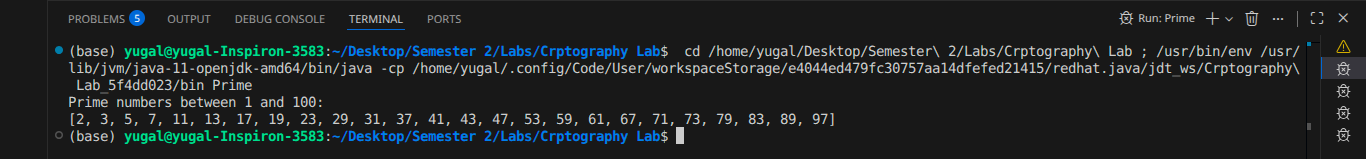
\includegraphics[width=1.0\textwidth]{Lab1/Images/program1.png}
    \caption{Program to print prime numbers between 1 and 1000}
    \label{fig:prime_number_output}
\end{figure}

%-----------------------------------------------
% Task 2
% -----------------------------------------------
\subsection{Write a program to perform matrix multiplication.}
\begin{lstlisting}[style=pythonStyle, caption={}]
import java.util.Scanner;

public class Matrix_Multiplication {

    public static void main(String[] args) {
        Scanner scanner = new Scanner(System.in);

        System.out.println("Enter the number of rows for the first matrix (A):");
        int rowsA = scanner.nextInt();
        System.out.println("Enter the number of columns for the first matrix (A):");
        int colsA = scanner.nextInt();

        System.out.println("Enter the number of rows for the second matrix (B):");
        int rowsB = scanner.nextInt();
        System.out.println("Enter the number of columns for the second matrix (B):");
        int colsB = scanner.nextInt();

        if (colsA != rowsB) {
            System.out.println("\nError: Matrix multiplication is not possible.");
            System.out.println("The number of columns in the first matrix must equal the number of rows in the second matrix.");
            return; 
        }

        int[][] matrixA = new int[rowsA][colsA];
        int[][] matrixB = new int[rowsB][colsB];
        int[][] resultMatrix = new int[rowsA][colsB];

        System.out.println("\nEnter elements of the first matrix (A):");
        for (int i = 0; i < rowsA; i++) {
            for (int j = 0; j < colsA; j++) {
                System.out.print("A[" + i + "][" + j + "]: ");
                matrixA[i][j] = scanner.nextInt();
            }
        }

        System.out.println("\nEnter elements of the second matrix (B):");
        for (int i = 0; i < rowsB; i++) {
            for (int j = 0; j < colsB; j++) {
                System.out.print("B[" + i + "][" + j + "]: ");
                matrixB[i][j] = scanner.nextInt();
            }
        }
  
        for (int i = 0; i < rowsA; i++) {
            for (int j = 0; j < colsB; j++) {
                for (int k = 0; k < colsA; k++) {
                    resultMatrix[i][j] += matrixA[i][k] * matrixB[k][j];
                }
            }
        }

        System.out.println("\nResultant Matrix:");
        for (int i = 0; i < rowsA; i++) {
            for (int j = 0; j < colsB; j++) {
                System.out.print(resultMatrix[i][j] + " ");
            }
            System.out.println(); 
        }

        scanner.close(); 
    }
}
\end{lstlisting}
\subsubsection*{Output}
% \vspace{-1em}
\begin{figure}[H]
    \centering
    \vspace{-1em}
    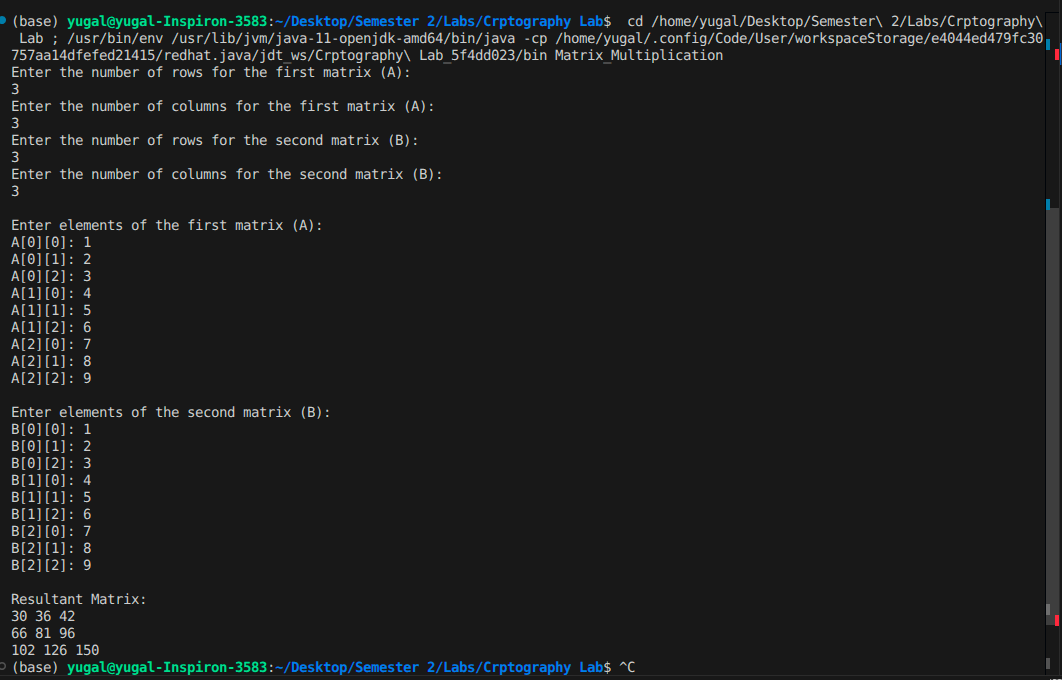
\includegraphics[width=1.0\textwidth]{Lab1/Images/program2.png}
    \caption{Program to perform matrix multiplication}
    \label{fig:matrix multiplication_output}
\end{figure}

%-----------------------------------------------
% Task 3
% -----------------------------------------------
\subsection{Write a program to find inverse of a matrix.}
\begin{lstlisting}[style=pythonStyle, caption={}]

import java.util.Scanner;

public class MatrixInverseSimple {

    public static void main(String[] args) {

        Scanner sc = new Scanner(System.in);

        double[][] a = new double[3][3];

        System.out.println("Enter elements of 3x3 matrix:");

        // Input
        for (int i = 0; i < 3; i++) {
            for (int j = 0; j < 3; j++) {
                a[i][j] = sc.nextDouble();
            }
        }

        // Determinant
        double det =
                a[0][0] * (a[1][1]*a[2][2] - a[1][2]*a[2][1])
              - a[0][1] * (a[1][0]*a[2][2] - a[1][2]*a[2][0])
              + a[0][2] * (a[1][0]*a[2][1] - a[1][1]*a[2][0]);

        if (det == 0) {
            System.out.println("Matrix is singular. No inverse.");
            return;
        }

        // Adjoint matrix
        double[][] adj = new double[3][3];

        adj[0][0] =  (a[1][1]*a[2][2] - a[1][2]*a[2][1]);
        adj[0][1] = -(a[0][1]*a[2][2] - a[0][2]*a[2][1]);
        adj[0][2] =  (a[0][1]*a[1][2] - a[0][2]*a[1][1]);

        adj[1][0] = -(a[1][0]*a[2][2] - a[1][2]*a[2][0]);
        adj[1][1] =  (a[0][0]*a[2][2] - a[0][2]*a[2][0]);
        adj[1][2] = -(a[0][0]*a[1][2] - a[0][2]*a[1][0]);

        adj[2][0] =  (a[1][0]*a[2][1] - a[1][1]*a[2][0]);
        adj[2][1] = -(a[0][0]*a[2][1] - a[0][1]*a[2][0]);
        adj[2][2] =  (a[0][0]*a[1][1] - a[0][1]*a[1][0]);

        // Inverse = adjoint / determinant
        System.out.println("Inverse Matrix:");

        for (int i = 0; i < 3; i++) {
            for (int j = 0; j < 3; j++) {
                System.out.printf("%6.2f ", adj[i][j] / det);
            }
            System.out.println();
        }

        sc.close();
    }
}
\end{lstlisting}
\subsubsection*{Output}
% \vspace{-1em}
\begin{figure}[H]
    \centering
    \vspace{-1em}
    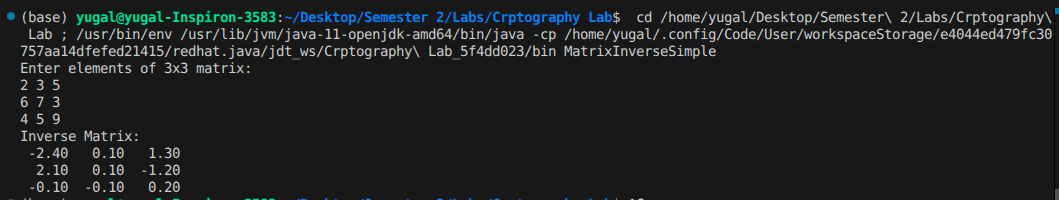
\includegraphics[width=1.0\textwidth]{Lab1/Images/program3.png}
    \caption{Program to find inverse of a matrix}
    \label{fig:matrix inverse_output}
\end{figure}

